\documentclass[11pt]{article}

\usepackage[margin=1in]{geometry}
\usepackage[T1]{fontenc}
\usepackage{graphicx}
\usepackage{longtable}
\usepackage{booktabs}
\usepackage{array}
\usepackage{enumitem}
\usepackage{xcolor}
\usepackage{hyperref}
\usepackage{tikz}
\usepackage{float}
\usepackage{fancyhdr}
\usepackage{titlesec}
\usepackage{tcolorbox}
\usepackage{tabularx}
\usepackage{multirow}
\usepackage{caption}
\usepackage{listings}
\usepackage{makecell}
\usepackage{amssymb}
\usepackage{pifont}

\usetikzlibrary{shapes.geometric, arrows.meta, positioning, fit, backgrounds, calc, decorations.pathreplacing, shapes.multipart, matrix, shadows}

% ---------------------------------------------------------------------------
% Color Definitions
% ---------------------------------------------------------------------------
\definecolor{sectionblue}{RGB}{31,78,121}
\definecolor{evalcolor}{RGB}{186,85,211}
\definecolor{businesscolor}{RGB}{255,165,0}
\definecolor{asrcolor}{RGB}{60,179,113}
\definecolor{riskcolor}{RGB}{220,53,69}
\definecolor{flowcolor}{RGB}{100,100,100}
\definecolor{lightgray}{RGB}{245,245,245}
\definecolor{warningred}{RGB}{220,53,69}
\definecolor{successgreen}{RGB}{40,167,69}
\definecolor{infoblue}{RGB}{23,162,184}
\definecolor{decisioncolor}{RGB}{70,130,180}
\definecolor{tradeoffcolor}{RGB}{255,127,80}
\definecolor{scenariocolor}{RGB}{144,238,144}
\definecolor{sensitivitycolor}{RGB}{255,182,193}

\hypersetup{
  colorlinks=true,
  linkcolor=sectionblue,
  urlcolor=sectionblue,
  citecolor=sectionblue
}

% ---------------------------------------------------------------------------
% Header and Footer
% ---------------------------------------------------------------------------
\pagestyle{fancy}
\fancyhf{}
\fancyhead[L]{\leftmark}
\fancyhead[R]{Supporting Evaluation Guide}
\fancyfoot[C]{\thepage}
\renewcommand{\headrulewidth}{0.4pt}
\renewcommand{\footrulewidth}{0.4pt}

% ---------------------------------------------------------------------------
% Section Formatting
% ---------------------------------------------------------------------------
\titleformat{\section}
  {\normalfont\Large\bfseries\color{sectionblue}}{\thesection}{1em}{}
\titleformat{\subsection}
  {\normalfont\large\bfseries\color{sectionblue!80}}{\thesubsection}{1em}{}
\titleformat{\subsubsection}
  {\normalfont\normalsize\bfseries\color{sectionblue!60}}{\thesubsubsection}{1em}{}

% ---------------------------------------------------------------------------
% Custom Box Environments
% ---------------------------------------------------------------------------
\newtcolorbox{keypoint}{
    colback=blue!5,
    colframe=sectionblue,
    title=Key Point,
    fonttitle=\bfseries
}

\newtcolorbox{warning}{
    colback=red!5,
    colframe=warningred,
    title=Warning,
    fonttitle=\bfseries
}

\newtcolorbox{bestpractice}{
    colback=green!5,
    colframe=successgreen,
    title=Best Practice,
    fonttitle=\bfseries
}

\newtcolorbox{example}{
    colback=lightgray,
    colframe=flowcolor,
    title=Example,
    fonttitle=\bfseries
}

\newtcolorbox{definition}{
    colback=infoblue!10,
    colframe=infoblue,
    title=Definition,
    fonttitle=\bfseries
}

\newtcolorbox{questionbox}[1][]{
    colback=evalcolor!10,
    colframe=evalcolor,
    title=#1,
    fonttitle=\bfseries,
    breakable
}

\newtcolorbox{businessbox}[1][]{
    colback=businesscolor!10,
    colframe=businesscolor,
    title=#1,
    fonttitle=\bfseries,
    breakable
}

\newtcolorbox{asrbox}[1][]{
    colback=asrcolor!10,
    colframe=asrcolor,
    title=#1,
    fonttitle=\bfseries
}

\newtcolorbox{riskbox}[1][]{
    colback=riskcolor!10,
    colframe=riskcolor,
    title=#1,
    fonttitle=\bfseries
}

\newtcolorbox{scenariobox}[1][]{
    colback=scenariocolor!15,
    colframe=asrcolor,
    title=#1,
    fonttitle=\bfseries
}

\newtcolorbox{checklistbox}[1][]{
    colback=white,
    colframe=flowcolor,
    title=#1,
    fonttitle=\bfseries
}

\newtcolorbox{decisionbox}[1][]{
    colback=decisioncolor!10,
    colframe=decisioncolor,
    title=#1,
    fonttitle=\bfseries
}

\tcbuselibrary{listings}

% ---------------------------------------------------------------------------
% List Settings
% ---------------------------------------------------------------------------
\setlist[itemize]{leftmargin=*,topsep=3pt,itemsep=2pt,parsep=0pt}
\setlist[enumerate]{leftmargin=*,topsep=3pt,itemsep=2pt,parsep=0pt}

% ---------------------------------------------------------------------------
% Custom Column Types
% ---------------------------------------------------------------------------
\newcolumntype{L}[1]{>{\raggedright\arraybackslash}p{#1}}
\newcolumntype{C}[1]{>{\centering\arraybackslash}p{#1}}
\newcolumntype{R}[1]{>{\raggedleft\arraybackslash}p{#1}}

% ---------------------------------------------------------------------------
% Custom Commands
% ---------------------------------------------------------------------------
\newcommand{\AD}{architecture description}
\newcommand{\ASR}{architecturally significant requirement}
\newcommand{\ASRs}{architecturally significant requirements}
\newcommand{\highprio}{\textcolor{riskcolor}{\textbf{H}}}
\newcommand{\medprio}{\textcolor{businesscolor}{\textbf{M}}}
\newcommand{\lowprio}{\textcolor{asrcolor}{\textbf{L}}}
\newcommand{\risk}{\textcolor{riskcolor}{\ding{72}}}
\newcommand{\sensitivity}{\textcolor{sensitivitycolor}{\ding{74}}}
\newcommand{\tradeoff}{\textcolor{tradeoffcolor}{\ding{73}}}

% ---------------------------------------------------------------------------
% Title
% ---------------------------------------------------------------------------
\title{%
    \vspace{-1cm}
    \textbf{\Huge Software Architecture Documentation}\\[12pt]
    \Large Supporting Evaluation\\[8pt]
    \large A Comprehensive Guide to Preparing Architecture Documentation\\
    for ATAM, CBAM, and Other Evaluation Methods
}
\author{%
    \textit{Architecture Documentation Series}\\[4pt]
    \small Based on SEI Evaluation Methods and Industry Best Practices
}
\date{\today}

\begin{document}
\maketitle
\thispagestyle{empty}

\vspace{0.5cm}

\begin{abstract}
\noindent
Architecture evaluation is a critical practice for assessing whether a software architecture will meet its intended quality goals before significant development investment. This comprehensive guide examines how architecture documentation supports formal evaluation methods such as ATAM (Architecture Tradeoff Analysis Method), CBAM (Cost Benefit Analysis Method), and ARID (Active Reviews for Intermediate Designs). The document provides detailed guidance on documenting business goals, architecturally significant requirements, quality attribute scenarios, architectural decisions, and risk/sensitivity analysis. Whether preparing for a formal evaluation or conducting internal architecture reviews, this guide ensures your documentation provides the analysis artifacts evaluators need.
\end{abstract}

\vfill

\begin{center}
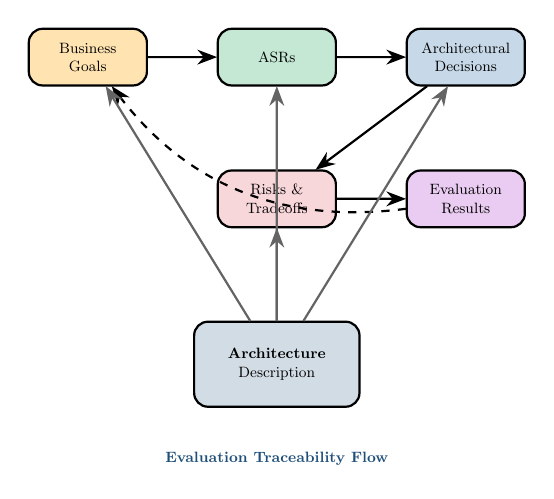
\begin{tikzpicture}[
    scale=0.6,
    transform shape,
    element/.style={draw, thick, rounded corners=5pt, minimum width=2.5cm, minimum height=1.2cm, font=\small, align=center},
    arrow/.style={-{Stealth[length=2.5mm]}, thick}
]
    % Flow from business to evaluation
    \node[element, fill=businesscolor!30] (business) at (0,4) {Business\\Goals};
    \node[element, fill=asrcolor!30] (asr) at (4,4) {ASRs};
    \node[element, fill=decisioncolor!30] (decision) at (8,4) {Architectural\\Decisions};
    \node[element, fill=riskcolor!20] (risk) at (4,1) {Risks \&\\Tradeoffs};
    \node[element, fill=evalcolor!30] (eval) at (8,1) {Evaluation\\Results};
    
    % Central AD
    \node[element, fill=sectionblue!20, minimum width=3.5cm, minimum height=1.8cm] (ad) at (4,-2.5) {\textbf{Architecture}\\Description};
    
    % Connections
    \draw[arrow] (business) -- (asr);
    \draw[arrow] (asr) -- (decision);
    \draw[arrow] (decision) -- (risk);
    \draw[arrow] (risk) -- (eval);
    \draw[arrow, dashed] (eval) to[bend left=30] (business);
    
    % AD connections
    \draw[arrow, flowcolor] (ad) -- (business);
    \draw[arrow, flowcolor] (ad) -- (asr);
    \draw[arrow, flowcolor] (ad) -- (decision);
    \draw[arrow, flowcolor] (ad) -- (risk);
    
    % Label
    \node[font=\bfseries\small, text=sectionblue] at (4,-4.5) {Evaluation Traceability Flow};
\end{tikzpicture}
\end{center}

\newpage
\tableofcontents
\newpage

%==============================================================================
\section{Introduction}
%==============================================================================

\subsection{Purpose of This Guide}

This guide examines how architecture documentation supports formal and informal architecture evaluation. Effective evaluation support ensures that:

\begin{itemize}
    \item Business goals and their architectural implications are clearly documented
    \item Architecturally significant requirements are identified, prioritized, and testable
    \item Architectural decisions and their rationale are captured
    \item Risks, sensitivities, and tradeoffs are identified and analyzed
    \item Evaluators can navigate from business goals through technical decisions to implications
    \item Evaluation results inform architectural refinement and business decisions
\end{itemize}

\subsection{What is Architecture Evaluation?}

\begin{definition}
\textbf{Architecture Evaluation:} A systematic examination of a software architecture to determine whether it will satisfy its quality attribute requirements, to identify risks and potential problems, and to assess tradeoffs among competing quality attributes.
\end{definition}

Architecture evaluation answers critical questions:
\begin{itemize}
    \item Will this architecture meet its quality goals?
    \item What are the risks in this architectural approach?
    \item What tradeoffs have been made and are they appropriate?
    \item Where are the sensitive points that require careful attention?
    \item Is the architecture suitable for the business context?
\end{itemize}

\subsection{Evaluation Methods Overview}

\begin{longtable}{@{}L{2.5cm} L{4.5cm} L{5.5cm}@{}}
\caption{Architecture Evaluation Methods} \\
\toprule
\textbf{Method} & \textbf{Purpose} & \textbf{Key Characteristics} \\
\midrule
\endfirsthead
\toprule
\textbf{Method} & \textbf{Purpose} & \textbf{Key Characteristics} \\
\midrule
\endhead
\bottomrule
\endlastfoot
ATAM & Identify risks, sensitivities, tradeoffs & Scenario-based; stakeholder-driven; quality attribute focus \\
CBAM & Cost-benefit analysis of architectural decisions & Economic analysis; ROI focus; builds on ATAM \\
ARID & Evaluate intermediate designs & Lightweight; design-focused; early feedback \\
SAAM & Analyze modifiability & Scenario-based; change-focused; predecessor to ATAM \\
ALMA & Analyze modifiability & Detailed change analysis; maintenance focus \\
Lightweight Methods & Quick risk identification & Reduced formality; faster execution; focused scope \\
\end{longtable}

\subsection{The Evaluation Traceability Chain}

Effective evaluation requires clear traceability from business goals to technical implementation:

\begin{figure}[H]
\centering
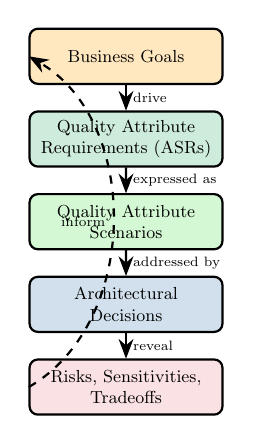
\begin{tikzpicture}[
    scale=0.7,
    transform shape,
    box/.style={draw, thick, fill=#1, minimum width=3.5cm, minimum height=1cm, rounded corners=3pt, font=\small, align=center},
    arrow/.style={-{Stealth[length=2.5mm]}, thick}
]
    \node[box=businesscolor!25] (bg) at (0,5) {Business Goals};
    \node[box=asrcolor!25] (asr) at (0,3.5) {Quality Attribute\\Requirements (ASRs)};
    \node[box=scenariocolor!40] (scen) at (0,2) {Quality Attribute\\Scenarios};
    \node[box=decisioncolor!25] (dec) at (0,0.5) {Architectural\\Decisions};
    \node[box=riskcolor!15] (risk) at (0,-1) {Risks, Sensitivities,\\Tradeoffs};
    
    \draw[arrow] (bg) -- node[right, font=\scriptsize] {drive} (asr);
    \draw[arrow] (asr) -- node[right, font=\scriptsize] {expressed as} (scen);
    \draw[arrow] (scen) -- node[right, font=\scriptsize] {addressed by} (dec);
    \draw[arrow] (dec) -- node[right, font=\scriptsize] {reveal} (risk);
    
    % Feedback
    \draw[arrow, dashed] (risk.west) to[bend right=60] node[left, font=\scriptsize] {inform} (bg.west);
\end{tikzpicture}
\caption{Evaluation Traceability Chain}
\end{figure}

%==============================================================================
\section{Business Goals and Drivers}
%==============================================================================

\subsection{Importance of Business Goals}

Architecture exists to serve business purposes. Evaluation must assess whether the architecture supports these purposes effectively.

\begin{keypoint}
\textbf{Business Goals Drive Architecture:}

Every architectural decision should trace back to one or more business goals. If a decision cannot be justified by business value, its necessity should be questioned.
\end{keypoint}

\subsection{Business Goal Categories}

\begin{longtable}{@{}L{3cm} L{4cm} L{5.5cm}@{}}
\caption{Business Goal Categories} \\
\toprule
\textbf{Category} & \textbf{Description} & \textbf{Examples} \\
\midrule
\endfirsthead
\toprule
\textbf{Category} & \textbf{Description} & \textbf{Examples} \\
\midrule
\endhead
\bottomrule
\endlastfoot
Revenue/Growth & Generate or increase revenue & New market entry; increased sales; premium features \\
Cost Reduction & Reduce operational or development costs & Automation; efficiency; reduced maintenance \\
Time to Market & Deliver capabilities faster & Rapid deployment; competitive response \\
Quality/Reliability & Ensure system dependability & High availability; data integrity; trust \\
Compliance & Meet regulatory requirements & GDPR; HIPAA; PCI-DSS; SOX \\
Competitive Advantage & Differentiate from competitors & Unique features; better performance; innovation \\
Risk Mitigation & Reduce business risks & Disaster recovery; security; vendor independence \\
Customer Satisfaction & Improve user experience & Usability; responsiveness; features \\
Operational Excellence & Improve operations & Scalability; maintainability; observability \\
Strategic Alignment & Support corporate strategy & Platform standardization; acquisition support \\
\end{longtable}

\subsection{Documenting Business Goals}

\begin{businessbox}[Business Goal Template]

\textbf{Goal ID:} [BG-XXX]

\textbf{Goal Statement:} [Clear, measurable statement of the business objective]

\textbf{Category:} [Revenue / Cost / Time / Quality / Compliance / etc.]

\textbf{Priority:} [Critical / High / Medium / Low]

\textbf{Stakeholder:} [Who owns or cares about this goal]

\textbf{Success Criteria:} [How we know the goal is achieved]

\textbf{Timeframe:} [When must this goal be achieved]

\textbf{Derived Quality Attributes:}
\begin{itemize}[nosep]
    \item [Quality attribute 1 and why it matters for this goal]
    \item [Quality attribute 2 and why it matters for this goal]
\end{itemize}

\textbf{Related ASRs:} [References to specific ASRs derived from this goal]

\textbf{Constraints:} [Business constraints affecting architectural choices]
\end{businessbox}

\subsection{Example Business Goals}

\begin{longtable}{@{}L{1.5cm} L{4cm} L{2cm} L{5cm}@{}}
\caption{Example Business Goals} \\
\toprule
\textbf{ID} & \textbf{Goal Statement} & \textbf{Priority} & \textbf{Derived Quality Attributes} \\
\midrule
\endfirsthead
\bottomrule
\endlastfoot
BG-001 & Support 100K concurrent users during peak events & \highprio{} Critical & Performance, Scalability, Availability \\
BG-002 & Enable new feature deployment in under 4 hours & \highprio{} Critical & Deployability, Modifiability, Testability \\
BG-003 & Achieve PCI-DSS Level 1 compliance & \highprio{} Critical & Security, Auditability \\
BG-004 & Reduce infrastructure costs by 30\% & \medprio{} High & Resource Efficiency, Elasticity \\
BG-005 & Enter European market within 12 months & \medprio{} High & Portability, Internationalization \\
BG-006 & Integrate with 3 major ERP systems & \medprio{} High & Interoperability, Integrability \\
\end{longtable}

%==============================================================================
\section{Architecturally Significant Requirements}
%==============================================================================

\subsection{What Makes a Requirement Architecturally Significant?}

\begin{definition}
An \textbf{Architecturally Significant Requirement (ASR)} is a requirement that has a profound effect on the architecture---that is, the architecture might be dramatically different in the absence of such a requirement.
\end{definition}

Requirements are architecturally significant when they:
\begin{itemize}
    \item Have a measurable effect on system structure
    \item Constrain design decisions significantly
    \item Affect multiple components or layers
    \item Are difficult or expensive to change later
    \item Require specific architectural tactics or patterns
    \item Have high business value and high technical risk
\end{itemize}

\subsection{ASR Sources}

\begin{figure}[H]
\centering
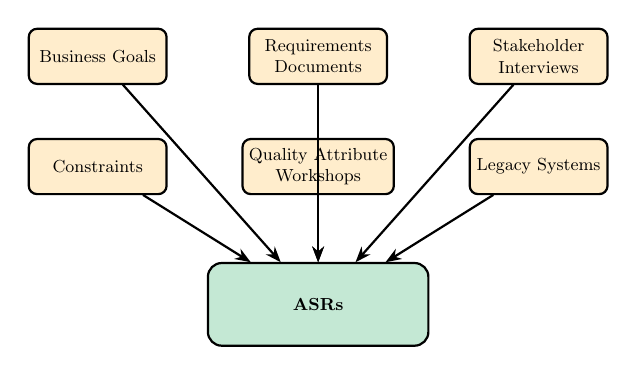
\begin{tikzpicture}[
    scale=0.7,
    transform shape,
    source/.style={draw, thick, fill=businesscolor!20, minimum width=2.5cm, minimum height=1cm, rounded corners=3pt, font=\small, align=center},
    asr/.style={draw, thick, fill=asrcolor!30, minimum width=4cm, minimum height=1.5cm, rounded corners=5pt, font=\small, align=center},
    arrow/.style={-{Stealth[length=2mm]}, thick}
]
    \node[source] (bg) at (-4,3) {Business Goals};
    \node[source] (req) at (0,3) {Requirements\\Documents};
    \node[source] (stake) at (4,3) {Stakeholder\\Interviews};
    \node[source] (const) at (-4,1) {Constraints};
    \node[source] (qa) at (0,1) {Quality Attribute\\Workshops};
    \node[source] (legacy) at (4,1) {Legacy Systems};
    
    \node[asr] (asrs) at (0,-1.5) {\textbf{ASRs}};
    
    \draw[arrow] (bg) -- (asrs);
    \draw[arrow] (req) -- (asrs);
    \draw[arrow] (stake) -- (asrs);
    \draw[arrow] (const) -- (asrs);
    \draw[arrow] (qa) -- (asrs);
    \draw[arrow] (legacy) -- (asrs);
\end{tikzpicture}
\caption{Sources of Architecturally Significant Requirements}
\end{figure}

\subsection{ASR Documentation Template}

\begin{asrbox}[ASR Documentation Template]

\textbf{ASR ID:} [ASR-XXX]

\textbf{Title:} [Brief descriptive title]

\textbf{Quality Attribute:} [Performance / Availability / Security / Modifiability / etc.]

\textbf{Source:} [Business goal, stakeholder, requirement document, etc.]

\textbf{Stimulus:} [What triggers this requirement]

\textbf{Environment:} [Context in which the stimulus occurs]

\textbf{Response:} [How the system should respond]

\textbf{Response Measure:} [Quantifiable measure of success]

\textbf{Priority:} [Critical / High / Medium / Low]

\textbf{Architectural Impact:}
\begin{itemize}[nosep]
    \item Affected components: [List of impacted elements]
    \item Required tactics: [Architectural tactics needed]
    \item Tradeoffs: [Other qualities that may be affected]
\end{itemize}

\textbf{Verification Method:} [How this ASR will be verified]

\textbf{Related Business Goals:} [BG-XXX, BG-YYY]

\textbf{Related Decisions:} [ADR-XXX, ADR-YYY]
\end{asrbox}

\subsection{ASR Prioritization}

\begin{longtable}{@{}L{2.5cm} C{2.5cm} C{2.5cm} L{5cm}@{}}
\caption{ASR Prioritization Matrix} \\
\toprule
\textbf{ASR} & \textbf{Business Value} & \textbf{Architectural Impact} & \textbf{Priority Rationale} \\
\midrule
\endfirsthead
\bottomrule
\endlastfoot
ASR-001 & High & High & Critical: Core business requirement with major structural impact \\
ASR-002 & High & Medium & High: Important business need, moderate architectural changes \\
ASR-003 & Medium & High & High: Significant architectural impact requiring early attention \\
ASR-004 & Medium & Medium & Medium: Balance of value and impact \\
ASR-005 & Low & High & Review: High impact but lower value---question necessity \\
ASR-006 & High & Low & Medium: Important but architecturally accommodated \\
\end{longtable}

%==============================================================================
\section{Quality Attribute Scenarios}
%==============================================================================

\subsection{What is a Quality Attribute Scenario?}

\begin{definition}
A \textbf{Quality Attribute Scenario} is a specific, testable statement of a quality attribute requirement. It consists of six parts: source, stimulus, artifact, environment, response, and response measure.
\end{definition}

Quality attribute scenarios make abstract quality requirements concrete and testable.

\subsection{Scenario Structure}

\begin{figure}[H]
\centering
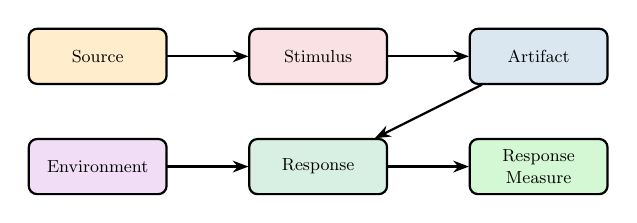
\begin{tikzpicture}[
    scale=0.7,
    transform shape,
    part/.style={draw, thick, fill=#1, minimum width=2.5cm, minimum height=1cm, rounded corners=3pt, font=\small, align=center},
    arrow/.style={-{Stealth[length=2mm]}, thick}
]
    \node[part=businesscolor!20] (source) at (-4,2) {Source};
    \node[part=riskcolor!15] (stimulus) at (0,2) {Stimulus};
    \node[part=decisioncolor!20] (artifact) at (4,2) {Artifact};
    \node[part=evalcolor!20] (env) at (-4,0) {Environment};
    \node[part=asrcolor!20] (response) at (0,0) {Response};
    \node[part=scenariocolor!40] (measure) at (4,0) {Response\\Measure};
    
    \draw[arrow] (source) -- (stimulus);
    \draw[arrow] (stimulus) -- (artifact);
    \draw[arrow] (artifact) -- (response);
    \draw[arrow] (env) -- (response);
    \draw[arrow] (response) -- (measure);
\end{tikzpicture}
\caption{Quality Attribute Scenario Structure}
\end{figure}

\begin{longtable}{@{}L{2.5cm} L{4cm} L{6cm}@{}}
\caption{Scenario Parts Explained} \\
\toprule
\textbf{Part} & \textbf{Description} & \textbf{Example} \\
\midrule
\endfirsthead
\bottomrule
\endlastfoot
Source & Origin of the stimulus & User, external system, internal process, attacker \\
Stimulus & Event that triggers the scenario & Request, failure, attack, change request \\
Artifact & System or component affected & Whole system, specific service, database \\
Environment & Context when stimulus occurs & Normal operation, peak load, degraded mode \\
Response & How system handles stimulus & Process request, recover, resist attack \\
Response Measure & Quantifiable outcome & Latency, recovery time, successful resistance \\
\end{longtable}

\subsection{Scenario Examples by Quality Attribute}

\begin{scenariobox}[Performance Scenario]
\textbf{Scenario ID:} QAS-PERF-001

\textbf{Source:} External user

\textbf{Stimulus:} Initiates a product search request

\textbf{Artifact:} Search Service

\textbf{Environment:} Normal operation with 10,000 concurrent users

\textbf{Response:} Search results returned to user

\textbf{Response Measure:} Within 200ms at 95th percentile
\end{scenariobox}

\begin{scenariobox}[Availability Scenario]
\textbf{Scenario ID:} QAS-AVAIL-001

\textbf{Source:} Internal infrastructure

\textbf{Stimulus:} Primary database server fails

\textbf{Artifact:} Order Processing System

\textbf{Environment:} Normal business hours

\textbf{Response:} System fails over to replica and continues processing

\textbf{Response Measure:} No more than 30 seconds of service interruption; no data loss
\end{scenariobox}

\begin{scenariobox}[Security Scenario]
\textbf{Scenario ID:} QAS-SEC-001

\textbf{Source:} External attacker

\textbf{Stimulus:} Attempts SQL injection attack on login form

\textbf{Artifact:} Authentication Service

\textbf{Environment:} Normal operation

\textbf{Response:} Attack detected, blocked, and logged; user session not compromised

\textbf{Response Measure:} 100\% of injection attempts blocked; alert generated within 1 second
\end{scenariobox}

\begin{scenariobox}[Modifiability Scenario]
\textbf{Scenario ID:} QAS-MOD-001

\textbf{Source:} Product team

\textbf{Stimulus:} Request to add new payment provider integration

\textbf{Artifact:} Payment Service

\textbf{Environment:} Design time

\textbf{Response:} New payment adapter implemented and deployed

\textbf{Response Measure:} Completed by one developer in 3 days; no changes to existing code
\end{scenariobox}

\subsection{Scenario Catalog Template}

\begin{longtable}{@{}L{1.5cm} L{2cm} L{3cm} L{3cm} L{2.5cm}@{}}
\caption{Quality Attribute Scenario Catalog} \\
\toprule
\textbf{ID} & \textbf{Quality} & \textbf{Stimulus} & \textbf{Response Measure} & \textbf{Priority} \\
\midrule
\endfirsthead
\toprule
\textbf{ID} & \textbf{Quality} & \textbf{Stimulus} & \textbf{Response Measure} & \textbf{Priority} \\
\midrule
\endhead
\bottomrule
\endlastfoot
QAS-001 & Performance & User search request & $<$200ms p95 & \highprio{} \\
QAS-002 & Performance & Checkout submission & $<$1s p99 & \highprio{} \\
QAS-003 & Availability & Database failure & $<$30s failover & \highprio{} \\
QAS-004 & Availability & Service crash & Auto-restart $<$10s & \highprio{} \\
QAS-005 & Security & SQL injection & 100\% blocked & \highprio{} \\
QAS-006 & Security & Brute force login & Lockout after 5 attempts & \medprio{} \\
QAS-007 & Modifiability & New payment provider & 3 person-days & \medprio{} \\
QAS-008 & Modifiability & UI framework change & 2 person-weeks & \lowprio{} \\
QAS-009 & Scalability & 10x load increase & Linear scaling & \medprio{} \\
QAS-010 & Testability & Unit test execution & $<$5 minutes & \medprio{} \\
\end{longtable}

%==============================================================================
\section{Architectural Decisions}
%==============================================================================

\subsection{Decision Documentation for Evaluation}

Evaluators need to understand what decisions were made, why they were made, and what alternatives were considered.

\begin{decisionbox}[Architecture Decision Record (ADR) for Evaluation]

\textbf{Decision ID:} [ADR-XXX]

\textbf{Title:} [Short descriptive title]

\textbf{Status:} [Proposed / Accepted / Deprecated / Superseded]

\textbf{Context:} [What is the issue or situation requiring a decision?]

\textbf{Decision Drivers:}
\begin{itemize}[nosep]
    \item [Business goal or ASR that drives this decision]
    \item [Constraint or force affecting the decision]
\end{itemize}

\textbf{Considered Alternatives:}

\textit{Option 1: [Name]}
\begin{itemize}[nosep]
    \item Description: [Brief description]
    \item Pros: [Advantages]
    \item Cons: [Disadvantages]
\end{itemize}

\textit{Option 2: [Name]}
\begin{itemize}[nosep]
    \item Description: [Brief description]
    \item Pros: [Advantages]
    \item Cons: [Disadvantages]
\end{itemize}

\textbf{Decision:} [What was decided]

\textbf{Rationale:} [Why this option was chosen]

\textbf{Consequences:}
\begin{itemize}[nosep]
    \item Positive: [Benefits of the decision]
    \item Negative: [Drawbacks or risks introduced]
    \item Neutral: [Other effects]
\end{itemize}

\textbf{Related ASRs:} [ASR-XXX, ASR-YYY]

\textbf{Related Decisions:} [ADR-XXX depends on / enables ADR-YYY]
\end{decisionbox}

\subsection{Example Decision Documentation}

\begin{example}
\textbf{ADR-003: Use Event-Driven Architecture for Inter-Service Communication}

\textbf{Context:} Services need to communicate state changes. We need loose coupling for independent deployment but also reliable message delivery.

\textbf{Decision Drivers:}
\begin{itemize}[nosep]
    \item BG-002: Enable rapid feature deployment
    \item ASR-003: Services must be independently deployable
    \item ASR-007: Support audit trail of all state changes
\end{itemize}

\textbf{Alternatives Considered:}
\begin{enumerate}[nosep]
    \item \textbf{Synchronous REST:} Simple but creates tight coupling
    \item \textbf{Event-Driven (Kafka):} Loose coupling, audit trail, complexity
    \item \textbf{Hybrid:} REST for queries, events for commands
\end{enumerate}

\textbf{Decision:} Event-driven architecture using Apache Kafka for all inter-service state changes.

\textbf{Rationale:} Provides loose coupling, natural audit trail, supports replay for debugging, and enables independent scaling. Complexity is acceptable given team experience.

\textbf{Consequences:}
\begin{itemize}[nosep]
    \item $(+)$ Services can be deployed independently
    \item $(+)$ Built-in audit trail through event log
    \item $(-)$ Eventual consistency requires careful handling
    \item $(-)$ Increased infrastructure complexity
\end{itemize}
\end{example}

\subsection{Decision Traceability Matrix}

\begin{longtable}{@{}L{2cm} L{3.5cm} L{3cm} L{4cm}@{}}
\caption{Decision Traceability Matrix} \\
\toprule
\textbf{Decision} & \textbf{Business Goals} & \textbf{ASRs Addressed} & \textbf{Scenarios Supported} \\
\midrule
\endfirsthead
\bottomrule
\endlastfoot
ADR-001 & BG-001, BG-004 & ASR-001, ASR-009 & QAS-001, QAS-009 \\
ADR-002 & BG-003 & ASR-005, ASR-006 & QAS-005, QAS-006 \\
ADR-003 & BG-002, BG-003 & ASR-003, ASR-007 & QAS-007 \\
ADR-004 & BG-001, BG-005 & ASR-001, ASR-002 & QAS-001, QAS-002, QAS-003 \\
ADR-005 & BG-004 & ASR-008, ASR-009 & QAS-009 \\
\end{longtable}

%==============================================================================
\section{Risk and Sensitivity Analysis}
%==============================================================================

\subsection{ATAM Analysis Outputs}

The Architecture Tradeoff Analysis Method (ATAM) produces specific analysis outputs:

\begin{longtable}{@{}L{3cm} L{3.5cm} L{6cm}@{}}
\caption{ATAM Analysis Outputs} \\
\toprule
\textbf{Output Type} & \textbf{Symbol} & \textbf{Description} \\
\midrule
\endfirsthead
\bottomrule
\endlastfoot
Risk & \risk{} & Architectural decision that may cause problems if wrong \\
Non-Risk & -- & Decision that is well-understood and acceptable \\
Sensitivity Point & \sensitivity{} & Property where small changes have large effects on quality \\
Tradeoff Point & \tradeoff{} & Property affecting multiple quality attributes in different ways \\
\end{longtable}

\subsection{Risk Documentation}

\begin{riskbox}[Risk Documentation Template]

\textbf{Risk ID:} [RISK-XXX]

\textbf{Title:} [Short descriptive title]

\textbf{Category:} [Technical / Business / Schedule / Resource]

\textbf{Description:} [What could go wrong]

\textbf{Source:} [Related decision, ASR, or scenario]

\textbf{Probability:} [High / Medium / Low]

\textbf{Impact:} [High / Medium / Low]

\textbf{Priority:} [Probability $\times$ Impact]

\textbf{Affected Quality Attributes:} [List of affected qualities]

\textbf{Affected Components:} [List of affected architectural elements]

\textbf{Mitigation Strategy:}
\begin{itemize}[nosep]
    \item [Action 1 to reduce risk]
    \item [Action 2 to reduce risk]
\end{itemize}

\textbf{Contingency Plan:} [What to do if the risk materializes]

\textbf{Owner:} [Who is responsible for monitoring/mitigation]

\textbf{Status:} [Open / Mitigated / Accepted / Closed]
\end{riskbox}

\subsection{Example Risks}

\begin{longtable}{@{}L{1.5cm} L{4cm} C{1.5cm} C{1.5cm} L{4cm}@{}}
\caption{Risk Register Example} \\
\toprule
\textbf{ID} & \textbf{Risk Description} & \textbf{Prob.} & \textbf{Impact} & \textbf{Mitigation} \\
\midrule
\endfirsthead
\bottomrule
\endlastfoot
RISK-001 & Event-driven system may have consistency issues under high load & Med & High & Implement idempotent handlers; add reconciliation jobs \\
RISK-002 & Single cloud provider dependency creates vendor lock-in & Low & High & Abstract cloud services; document migration path \\
RISK-003 & Microservice complexity may slow initial development & High & Med & Start with fewer services; split as needed \\
RISK-004 & Performance targets may not be achievable with chosen database & Med & High & Conduct early performance testing; have backup plan \\
RISK-005 & Team lacks experience with chosen event streaming platform & Med & Med & Training; hire consultant; start with simple patterns \\
\end{longtable}

\subsection{Sensitivity Points}

\begin{longtable}{@{}L{1.5cm} L{4cm} L{3cm} L{4cm}@{}}
\caption{Sensitivity Points} \\
\toprule
\textbf{ID} & \textbf{Sensitivity Point} & \textbf{Affected Quality} & \textbf{Implications} \\
\midrule
\endfirsthead
\bottomrule
\endlastfoot
SP-001 & Database connection pool size & Performance & Too small: timeouts; Too large: resource exhaustion \\
SP-002 & Cache TTL settings & Performance, Consistency & Short: more DB load; Long: stale data \\
SP-003 & Circuit breaker thresholds & Availability, Performance & Sensitive: false positives; Lenient: cascading failures \\
SP-004 & Event partition count & Scalability, Performance & Too few: bottleneck; Too many: overhead \\
SP-005 & Retry attempt limits & Availability, Resource usage & Few: premature failure; Many: resource exhaustion \\
\end{longtable}

\subsection{Tradeoff Points}

\begin{longtable}{@{}L{1.5cm} L{3.5cm} L{3cm} L{4.5cm}@{}}
\caption{Tradeoff Points} \\
\toprule
\textbf{ID} & \textbf{Tradeoff Point} & \textbf{Qualities Affected} & \textbf{Tradeoff Description} \\
\midrule
\endfirsthead
\bottomrule
\endlastfoot
TP-001 & Synchronous vs. async communication & Performance $\leftrightarrow$ Consistency & Async improves performance but introduces eventual consistency \\
TP-002 & Caching strategy & Performance $\leftrightarrow$ Freshness & More caching improves performance but data may be stale \\
TP-003 & Service granularity & Modifiability $\leftrightarrow$ Performance & Fine-grained services are more modifiable but have more overhead \\
TP-004 & Encryption level & Security $\leftrightarrow$ Performance & Stronger encryption improves security but impacts performance \\
TP-005 & Logging verbosity & Debuggability $\leftrightarrow$ Performance & More logging helps debugging but impacts performance \\
\end{longtable}

%==============================================================================
\section{Views for Evaluation}
%==============================================================================

\subsection{View-to-ASR Mapping}

Evaluators need to know which views address which quality attributes:

\begin{longtable}{@{}L{2.5cm} L{4cm} L{6cm}@{}}
\caption{View-to-Quality Attribute Mapping} \\
\toprule
\textbf{View Type} & \textbf{Primary Quality Attributes} & \textbf{Evaluation Use} \\
\midrule
\endfirsthead
\bottomrule
\endlastfoot
Module Decomposition & Modifiability, Testability, Reusability & Change impact analysis; team allocation \\
Uses/Dependencies & Modifiability, Buildability & Build dependencies; change propagation \\
Layered & Portability, Modifiability & Abstraction analysis; dependency rules \\
Component-Connector & Performance, Availability, Security & Runtime analysis; communication paths \\
Deployment & Availability, Performance, Security & Resource allocation; failure analysis \\
Data Model & Performance, Security, Consistency & Data access patterns; integrity analysis \\
\end{longtable}

\subsection{View Completeness for Evaluation}

\begin{checklistbox}[View Completeness Checklist for Evaluation]

\textbf{For Each ASR, verify:}
\begin{itemize}[leftmargin=1.5cm]
    \item[$\square$] At least one view addresses the ASR
    \item[$\square$] View provides sufficient detail for analysis
    \item[$\square$] Relevant architectural tactics are visible
    \item[$\square$] Related decisions are documented
\end{itemize}

\textbf{For Each View, verify:}
\begin{itemize}[leftmargin=1.5cm]
    \item[$\square$] View purpose and stakeholders identified
    \item[$\square$] Notation clearly explained
    \item[$\square$] Models are complete for intended analysis
    \item[$\square$] Assumptions and limitations documented
\end{itemize}

\textbf{For Cross-View Analysis:}
\begin{itemize}[leftmargin=1.5cm]
    \item[$\square$] Correspondences between views documented
    \item[$\square$] Consistency between views verified
    \item[$\square$] Combined analysis is possible
\end{itemize}
\end{checklistbox}

%==============================================================================
\section{Review Question Sets}
%==============================================================================

\subsection{Questions for Business Managers}

\begin{questionbox}[Business Manager Questions]

\textbf{Business Goals:}
\begin{enumerate}
    \item Are the business goals the system must satisfy clearly articulated?
    \begin{itemize}[nosep]
        \item Where are business goals documented?
        \item Are they stated in measurable terms?
    \end{itemize}
    
    \item Are business goals prioritized?
    \begin{itemize}[nosep]
        \item Who determined priorities?
        \item What criteria were used for prioritization?
    \end{itemize}
    
    \item Are success criteria defined for each business goal?
    \begin{itemize}[nosep]
        \item How will success be measured?
        \item What is the timeframe for achievement?
    \end{itemize}
\end{enumerate}

\textbf{Goal-to-Architecture Traceability:}
\begin{enumerate}[resume]
    \item Is there clear mapping between business goals and requirements?
    \begin{itemize}[nosep]
        \item Can you trace from each goal to specific requirements?
        \item Are requirements prioritized according to business importance?
    \end{itemize}
    
    \item Can you navigate from business goals to technical decisions?
    \begin{itemize}[nosep]
        \item Are the connections documented?
        \item Is the rationale for decisions clear?
    \end{itemize}
    
    \item Can you trace from technical decisions back to business implications?
    \begin{itemize}[nosep]
        \item Do you understand risks to business goals?
        \item Are tradeoffs that affect business clearly identified?
    \end{itemize}
\end{enumerate}

\textbf{Criteria and Evolution:}
\begin{enumerate}[resume]
    \item What criteria determine whether architecture supports business goals?
    \begin{itemize}[nosep]
        \item Are criteria documented?
        \item How will criteria be evaluated?
    \end{itemize}
    
    \item How might the system change over its deployment lifetime?
    \begin{itemize}[nosep]
        \item What business changes are anticipated?
        \item Is retirement/replacement considered?
    \end{itemize}
\end{enumerate}
\end{questionbox}

\subsection{Questions for Architects}

\begin{questionbox}[Architect Questions]

\textbf{Context and Stakeholders:}
\begin{enumerate}
    \item Is the system context clearly defined?
    \begin{itemize}[nosep]
        \item External systems and interfaces identified?
        \item Boundaries clearly established?
    \end{itemize}
    
    \item Have stakeholders and their concerns been defined?
    \begin{itemize}[nosep]
        \item Is the stakeholder list complete?
        \item Are concerns mapped to stakeholders?
    \end{itemize}
\end{enumerate}

\textbf{Requirements and ASRs:}
\begin{enumerate}[resume]
    \item Have requirements, constraints, and standards been defined?
    \begin{itemize}[nosep]
        \item Functional requirements documented?
        \item Quality requirements documented?
        \item Constraints clearly stated?
    \end{itemize}
    
    \item Are ASRs clearly articulated and prioritized?
    \begin{itemize}[nosep]
        \item What makes each requirement architecturally significant?
        \item How was prioritization determined?
    \end{itemize}
    
    \item Are ASRs clear, unambiguous, and testable?
    \begin{itemize}[nosep]
        \item Are quality attribute scenarios defined?
        \item Are response measures quantified?
    \end{itemize}
\end{enumerate}

\textbf{Decisions and Rationale:}
\begin{enumerate}[resume]
    \item Are techniques used to achieve ASRs documented?
    \begin{itemize}[nosep]
        \item What architectural tactics were applied?
        \item What patterns were used?
    \end{itemize}
    
    \item Have alternatives been considered and documented?
    \begin{itemize}[nosep]
        \item What options were evaluated?
        \item Why were alternatives rejected?
    \end{itemize}
    
    \item Are key decisions identified and located?
    \begin{itemize}[nosep]
        \item Where is the decision log?
        \item Are decisions traceable to ASRs?
    \end{itemize}
    
    \item Is rationale captured for key decisions?
    \begin{itemize}[nosep]
        \item Is reasoning documented?
        \item Are tradeoffs explained?
    \end{itemize}
\end{enumerate}

\textbf{Analysis Artifacts:}
\begin{enumerate}[resume]
    \item Can you describe runtime resources for each operational concern?
    \begin{itemize}[nosep]
        \item CPU, memory, network, storage requirements?
        \item Resource allocation rationale?
    \end{itemize}
    
    \item Can you describe change impact for modifiability concerns?
    \begin{itemize}[nosep]
        \item Size and difficulty of anticipated changes?
        \item Components affected by changes?
    \end{itemize}
    
    \item Can you determine views necessary to analyze each ASR?
    \begin{itemize}[nosep]
        \item Which views address which ASRs?
        \item Are views sufficient for analysis?
    \end{itemize}
    
    \item Do models within views address ASRs adequately?
    \begin{itemize}[nosep]
        \item Is there enough information to evaluate ASR satisfaction?
        \item Are gaps identified?
    \end{itemize}
    
    \item Are all ASRs addressed by models or correspondences?
    \begin{itemize}[nosep]
        \item Is coverage complete?
        \item Are any ASRs unaddressed?
    \end{itemize}
\end{enumerate}

\textbf{Preliminary Analysis:}
\begin{enumerate}[resume]
    \item Have architects conducted preliminary analysis?
    \begin{itemize}[nosep]
        \item What analysis has been done?
        \item Where are results documented?
    \end{itemize}
    
    \item Are risks and issues articulated?
    \begin{itemize}[nosep]
        \item Is there a risk register?
        \item Are sensitivity and tradeoff points identified?
    \end{itemize}
\end{enumerate}

\textbf{Completeness and Navigation:}
\begin{enumerate}[resume]
    \item Is the documentation complete?
    \begin{itemize}[nosep]
        \item Are placeholders identified for incomplete items?
        \item Is there a completion plan?
    \end{itemize}
    
    \item Can you navigate through material during evaluation?
    \begin{itemize}[nosep]
        \item Can you show decisions for stakeholder concerns?
        \item Are cross-references accurate?
    \end{itemize}
\end{enumerate}
\end{questionbox}

\subsection{Questions for Evaluation Team}

\begin{questionbox}[Evaluation Team Questions]

\textbf{Documentation Clarity:}
\begin{enumerate}
    \item Are concepts and notations clearly explained?
    \begin{itemize}[nosep]
        \item Is there a glossary of terms?
        \item Is there a key for diagrams?
        \item Is notation consistent throughout?
    \end{itemize}
\end{enumerate}

\textbf{Evaluation Scope:}
\begin{enumerate}[resume]
    \item Have evaluation scope and objectives been defined?
    \begin{itemize}[nosep]
        \item What is being evaluated?
        \item What are the evaluation goals?
        \item What is out of scope?
    \end{itemize}
    
    \item Is the system context for evaluation clearly defined?
    \begin{itemize}[nosep]
        \item Boundaries of evaluation clear?
        \item External dependencies identified?
    \end{itemize}
    
    \item Have stakeholders and concerns for evaluation been identified?
    \begin{itemize}[nosep]
        \item Who should participate?
        \item What concerns will be evaluated?
    \end{itemize}
\end{enumerate}

\textbf{View Evaluation:}
\begin{enumerate}[resume]
    \item For each view, do you understand how to evaluate it?
    \begin{itemize}[nosep]
        \item Is the evaluation approach clear?
        \item Are analysis techniques applicable?
    \end{itemize}
    
    \item For correspondences across views, do you understand representation?
    \begin{itemize}[nosep]
        \item How are correspondences documented?
        \item How will you evaluate accuracy and completeness?
    \end{itemize}
    
    \item Are views sufficiently complete for intended analysis?
    \begin{itemize}[nosep]
        \item What gaps exist?
        \item Can you work around identified gaps?
    \end{itemize}
\end{enumerate}

\textbf{Analysis Preparation:}
\begin{enumerate}[resume]
    \item Is the quality attribute scenario list complete and prioritized?
    \begin{itemize}[nosep]
        \item Are scenarios testable?
        \item Do scenarios cover key quality concerns?
    \end{itemize}
    
    \item Can you identify architectural approaches for each scenario?
    \begin{itemize}[nosep]
        \item Are tactics visible in the architecture?
        \item Can you trace scenarios to decisions?
    \end{itemize}
    
    \item Can you identify potential risks, sensitivities, and tradeoffs?
    \begin{itemize}[nosep]
        \item Where might problems occur?
        \item What are the sensitive parameters?
        \item What competing qualities exist?
    \end{itemize}
\end{enumerate}
\end{questionbox}

%==============================================================================
\section{Evaluation Readiness Assessment}
%==============================================================================

\subsection{Readiness Checklist}

\begin{checklistbox}[Architecture Evaluation Readiness Checklist]

\textbf{Business Context:}
\begin{itemize}[leftmargin=1.5cm]
    \item[$\square$] Business goals documented
    \item[$\square$] Goals prioritized
    \item[$\square$] Success criteria defined
    \item[$\square$] Goal-to-requirement traceability exists
\end{itemize}

\textbf{ASRs and Scenarios:}
\begin{itemize}[leftmargin=1.5cm]
    \item[$\square$] ASRs identified and documented
    \item[$\square$] ASRs prioritized by architectural impact
    \item[$\square$] Quality attribute scenarios defined
    \item[$\square$] Scenarios are testable with response measures
\end{itemize}

\textbf{Architectural Decisions:}
\begin{itemize}[leftmargin=1.5cm]
    \item[$\square$] Key decisions identified
    \item[$\square$] Alternatives considered and documented
    \item[$\square$] Rationale captured for each decision
    \item[$\square$] Decision-to-ASR traceability exists
\end{itemize}

\textbf{Analysis Artifacts:}
\begin{itemize}[leftmargin=1.5cm]
    \item[$\square$] Risks identified
    \item[$\square$] Sensitivity points identified
    \item[$\square$] Tradeoff points identified
    \item[$\square$] Preliminary analysis documented
\end{itemize}

\textbf{Views and Models:}
\begin{itemize}[leftmargin=1.5cm]
    \item[$\square$] Views address all ASRs
    \item[$\square$] View notation explained
    \item[$\square$] Models complete for analysis
    \item[$\square$] Cross-view correspondences documented
\end{itemize}

\textbf{Documentation Quality:}
\begin{itemize}[leftmargin=1.5cm]
    \item[$\square$] Glossary of terms provided
    \item[$\square$] Diagram keys provided
    \item[$\square$] Navigation aids in place
    \item[$\square$] Gaps identified with placeholders
\end{itemize}
\end{checklistbox}

\subsection{Readiness Assessment Matrix}

\begin{longtable}{@{}L{3.5cm} C{1.5cm} C{1.5cm} C{1.5cm} L{4cm}@{}}
\caption{Evaluation Readiness Assessment} \\
\toprule
\textbf{Criterion} & \textbf{Ready} & \textbf{Partial} & \textbf{Not Ready} & \textbf{Notes} \\
\midrule
\endfirsthead
\bottomrule
\endlastfoot
Business goals documented & $\square$ & $\square$ & $\square$ & \\
Goals prioritized & $\square$ & $\square$ & $\square$ & \\
ASRs identified & $\square$ & $\square$ & $\square$ & \\
ASRs prioritized & $\square$ & $\square$ & $\square$ & \\
Scenarios defined & $\square$ & $\square$ & $\square$ & \\
Scenarios testable & $\square$ & $\square$ & $\square$ & \\
Decisions documented & $\square$ & $\square$ & $\square$ & \\
Alternatives considered & $\square$ & $\square$ & $\square$ & \\
Rationale captured & $\square$ & $\square$ & $\square$ & \\
Risks identified & $\square$ & $\square$ & $\square$ & \\
Views cover ASRs & $\square$ & $\square$ & $\square$ & \\
Notation explained & $\square$ & $\square$ & $\square$ & \\
\midrule
\textbf{Overall Readiness} & $\square$ & $\square$ & $\square$ & \\
\end{longtable}

%==============================================================================
\section{Appendix A: ATAM Overview}
%==============================================================================

\begin{keypoint}
\textbf{Architecture Tradeoff Analysis Method (ATAM)}

ATAM is the most widely used architecture evaluation method, developed by the Software Engineering Institute (SEI). It provides a structured approach for evaluating software architectures against quality attribute requirements.
\end{keypoint}

\subsection{ATAM Phases}

\begin{longtable}{@{}L{2.5cm} L{3.5cm} L{6.5cm}@{}}
\caption{ATAM Phases and Activities} \\
\toprule
\textbf{Phase} & \textbf{Activities} & \textbf{Documentation Needed} \\
\midrule
\endfirsthead
\bottomrule
\endlastfoot
Phase 0: Partnership & Define scope; identify stakeholders; plan evaluation & Stakeholder list; evaluation scope; schedule \\
Phase 1: Evaluation & Present business drivers; present architecture; identify approaches; analyze scenarios & Business goals; architecture overview; architectural approaches; utility tree \\
Phase 2: Evaluation & Brainstorm scenarios; prioritize scenarios; analyze scenarios; present results & Refined scenarios; analysis results; risks, sensitivities, tradeoffs \\
Phase 3: Follow-up & Document results; track findings & Final report; action items \\
\end{longtable}

\subsection{ATAM Outputs}

\begin{itemize}
    \item \textbf{Architectural approaches:} Key design strategies identified
    \item \textbf{Quality attribute utility tree:} Hierarchical view of quality requirements
    \item \textbf{Prioritized scenarios:} Scenarios ranked by importance
    \item \textbf{Risk themes:} Patterns of risks across the architecture
    \item \textbf{Sensitivity points:} Parameters with significant impact
    \item \textbf{Tradeoff points:} Competing quality attribute effects
    \item \textbf{Risks and non-risks:} Evaluated architectural decisions
\end{itemize}

%==============================================================================
\section{Appendix B: Quality Attribute Scenario Template}
%==============================================================================

\begin{scenariobox}[Quality Attribute Scenario Template]

\textbf{Scenario ID:} [QAS-XXX]

\textbf{Quality Attribute:} [e.g., Performance, Security, Availability]

\textbf{Business Goal:} [BG-XXX - Related business goal]

\textbf{ASR:} [ASR-XXX - Related ASR]

\textbf{Source of Stimulus:} [Who or what generates the stimulus]

\textbf{Stimulus:} [The condition or event]

\textbf{Artifact:} [What part of system is affected]

\textbf{Environment:} [Operating conditions]

\textbf{Response:} [How system should behave]

\textbf{Response Measure:} [Quantifiable measure]

\textbf{Priority:} [H/M/L based on business importance and architectural impact]

\textbf{Architectural Approach:} [How architecture addresses this scenario]

\textbf{Analysis Notes:} [Preliminary analysis, risks, concerns]
\end{scenariobox}

%==============================================================================
\section{Appendix C: Glossary}
%==============================================================================

\begin{description}[leftmargin=3cm, style=nextline]
    \item[Architectural Approach] A collection of architectural decisions that address one or more quality attributes
    \item[Architecturally Significant Requirement (ASR)] A requirement that has measurable impact on system architecture
    \item[ATAM] Architecture Tradeoff Analysis Method; structured approach for evaluating architectures
    \item[Business Goal] A statement of organizational objective the system must support
    \item[CBAM] Cost Benefit Analysis Method; economic analysis of architectural decisions
    \item[Quality Attribute] A measurable property of a system (e.g., performance, security)
    \item[Quality Attribute Scenario] A testable specification of a quality requirement
    \item[Risk] An architectural decision that may lead to undesirable consequences
    \item[Sensitivity Point] An architectural parameter where small changes have large effects
    \item[Tradeoff Point] An architectural decision affecting multiple qualities differently
    \item[Utility Tree] A hierarchical representation of quality attribute requirements
\end{description}

%==============================================================================
\section{Appendix D: References}
%==============================================================================

\begin{enumerate}
    \item Clements, P., Kazman, R., \& Klein, M. (2002). \textit{Evaluating Software Architectures: Methods and Case Studies}. Addison-Wesley.
    
    \item Bass, L., Clements, P., \& Kazman, R. (2021). \textit{Software Architecture in Practice} (4th ed.). Addison-Wesley.
    
    \item Kazman, R., Klein, M., \& Clements, P. (2000). \textit{ATAM: Method for Architecture Evaluation}. CMU/SEI-2000-TR-004.
    
    \item Kazman, R., Asundi, J., \& Klein, M. (2001). \textit{Quantifying the Costs and Benefits of Architectural Decisions}. ICSE 2001.
    
    \item Clements, P., et al. (2010). \textit{Documenting Software Architectures: Views and Beyond} (2nd ed.). Addison-Wesley.
    
    \item Rozanski, N., \& Woods, E. (2011). \textit{Software Systems Architecture} (2nd ed.). Addison-Wesley.
    
    \item ISO/IEC/IEEE 42030:2019. \textit{Software, systems and enterprise---Architecture evaluation framework}.
    
    \item Barbacci, M., et al. (2003). \textit{Quality Attribute Workshops (QAWs), Third Edition}. CMU/SEI-2003-TR-016.
\end{enumerate}

\end{document}